\section{Ejercicio 2}
\subsection{Problema}
Dise\~nar e implementar un \textbf{algoritmo exacto} para List Coloring y desarrollar los siguientes puntos:\\

a) Explicar detalladamente el algoritmo implementado. Elaborar podas y estrategias que permitan mejorar los tiempos de ejecuci\'on. En los casos en los que el backtracking reduzca el problema a 2-List Coloring utilizar el algoritmo del item anterior como caso base.\\

b) Calcular el orden de complejidad temporal de peor caso del algoritmo.\\

c) Realizar una experimentaci\'on que permita observar los tiempos de ejecuci\'on del algoritmo en funci\'on del tama\~no de entrada y de las podas y/o estrategias implementadas.\\

\subsection{Explicaci\'on y desarrollo del problema}
Como vimos en clase, no se conoce ningun algortimo de orden polinomial para resolver este problema. Si bien no podremos mejorar la cota exponencial del algoritmo, nuestro objetivo estara en realizar un backtracking inteligente y distintas podas que ayuden a recortar el arbol de recursion y por ende achicar los tiempos de ejecucion. 

Recordemos que.. Backtracking(subsoluci\'on $s$):
\begin{itemize}
\item Si $s$ es invalido $\Rightarrow$ Falso
\item Si es $s$ valido $\Rightarrow$ res $<-s$ y Terminar
\item Si no, elegir una decicion D que falte tomar y para cada posible eleccion E de D, Backtracking($s+e$)
\end{itemize}
A este esquema la agregaremos dos tipos de podas. Una poda es una manera mas de saber cuando estamos en una subsolucion invalida.\\
La primera consiste en chequear si dada una materia A, pintada del color C, existe algun vecino tal que su unico color disponible es C. En ese caso sabemos que tendremos un conflicto ya que no podemos tener dos vecinos pintados del mismo color. Al encontrarnos con un conflictos, es en vano seguir por esa rama del backtracking por lo que decimos que el resultado de ir por ese lado es false y volvemos la recursion hacia atras.\\
La segunda poda es un poco mas compleja. Esta consiste en fijarse si existe un color disponible para mi materia tal que ese color no este diponible para ningun vecino. De esta manera, sabremos que esa materia puede pintarse exactamente de ese color y que no tendra ningun conflicto con sus vecinos (ya que como dijimos recien, ningun vecino tiene ese color). La implementacion va de la siguiente manera: Sea N la materia donde nos encontramos, preguntaremos si #(colores(N)) es mayor a #(colores(N)\ $\cap$ (vecinos(N)).\\
Esto quiere decir que existe un color K en N tal que no esta en ninguno de sus vecinos por ende puedo pintar automaticamente el nodo de color K.

%!% = Linea demasiado javaStyle para mi. Damian . tenias que escapear el "\cap"
\subsection{Pseudo-C\'odigo}
\begin{verbatim}


solverWithBacktrack()
    ArrayList<NodoMateria> nodos = new ArrayList<NodoMateria>();%!%
    ejercicio1 = new Ejercicio1(grafo.size());%!%
    FOREACH Materias(grafo) AS nodoMateria
        IF #ColoresPosibles(nodoMateria) > 2 THEN
            Agregar(nodoMateria, nodos)
         ELSE 
            FOR color desde 0 hasta ColoresPosibles(nodoMateria)
                Setearcolor(color,nodoMateria)
                ENDFOR
        ENDIF
    ENDFOR
    IF VACIO?(nodos) THEN
        RES = (solucion = ejercicio1.solve(grafo)) != NULL)%!%
    ELSE
        RES = backTrack(nodos);            
    ENDIF

backTrack(ArrayList<NodoMateria> materiasColores){
    NodoMateria materia = materiasColores.get(0)%!%
    materiasColores.remove(0);%!%
    bool solucion = false
    int i = 0
    
    IF poda2(materia) != -1 THEN
        materia.setColor(materia.getColores().get(i)); %!%
        if (backTrack(materiasColores))
            RES = true
        ENDIF
    ELSE 
            WHILE (i < #Colores(materia) || ! solucion)
                materia.setColor(materia.getColores().get(i)); %!%
                IF (poda1(materia,materia.getColores().get(i)))%!%
                    if #MateriasColores == 0 THEN
                        IF ejercicio1.solve() THEN 
                            RES = true
                        ELSE 
                            IF backTrack(materiasColores) THEN
                            RES = true
                            ENDIF
                        ENDIF        
                    ENDIF
                ENDIF
            ENDWHILE
    ENDIF
    RES = ejercicio1.solve
}
    
boolean poda1(NodoMateria materia, int color){
    FOREACH vecino(materia) AS materiaVecina
        IF #(Colores(materiaVecina)) == 1 && color PERTENECEA Colores(materiaVecina) THEN
            RES = false
        ENDIF
    ENDFOR
    
    RES = true
}
    
Integer poda2(NodoMateria materia){
    ArrayList<Integer> coloresPosibles = new ArrayList<Integer>(materia.getColores());%!%
    ArrayList<Integer> coloresVecinos  = new ArrayList<Integer>();%!%

    FOREACH Vecinos(materia) AS materiaVecina
        AgregarTodos(colores(materiaVecina), coloresVecinos)
    ENDFOREACH
    
    coloresPosibles.retainAll(coloresVecinos);%!%
    IF #coloresPosibles == #Colores(materia)
        RES = -1
        ELSE 
        FOR i desde 0 hasta #(Colores(materia)) 
            IF (!coloresPosibles.contains(materia.getColores().get(i)))%!%
                RES = materia.getColores().get(i);%!%
            ENDIF
        ENDFOR
    ENDIF
    
    RES = -1
}

solverWithBacktrack()
    nodos <- lista<Nodos>
    ejercicio1 <- InstanciaEj1(tamaño(grafo))
    
    FOREACH materias(grafo) AS  nodoMateria
        IF coloresPosibles(nodoMateria) > 2 THEN
            agregar(nodos,nodoMateria)
        ELSE
            FOREACH coloresPosibles(nodoMateria) AS color
                nodoMateria.setColor(color)
            ENDFOREACH
        ENDIF
    ENDFOREACH

    IF nodos.isEmpty() THEN
        DEVOLVER ejercicio1.solve(grafo)
    ELSE
        DEVOLVER backTrack(nodos)
    ENDIF

private boolean backTrack(ArrayList<NodoMateria> materiasColores){
    NodoMateria materia = desencolar(materiasColores)
    boolean tieneSolucion = false;
    int i = 0;
    IF poda2(materia) != -1 THEN
    materia.setColor(materia.getColores().get(i)); // Seteo el color de backtrack
    IF tamano(materiasColores) == 0 THEN
        IF ((solucion = ejercicio1.solve(grafo)) != null){
            DEVOLVER true;
        ENDIF
    ELSE
        IF backTrack(materiasColores)
            DEVOLVER true
        ENDIF
    ENDIF
    materia.clearColors()
    ELSE
        WHILE i < coloresPosibles(materia) ^ !tieneSolucion DO
    
            materia.setColor(materia.getColorPosible(i))
    
            IF (poda1(materia,materia.getColorPosible(i))){
                IF ((solucion = ejercicio1.solve(grafo)) != null){
                    DEVOLVER true;
                ENDIF
            ELSE
                IF backTrack(materiasColores)
                    DEVOLVER true
                ENDIF
            ENDIF
            i++;
            materia.clearColors();
            ENDIF
        ENDWHILE
    ENDIF
    materiasColores.add(0,materia);
    DEVOLVER false

\end{verbatim}
\pagebreak
\subsection{Justificaci\'on y Complejidad}
Como explicamos antes, no se conocen algoritmos en orden polinomial para resolver el problema por lo que nuestro algoritmo tiene una complejidad exponencial. Esta viene dada por el backtracking, el hecho de que explore todas las posibles combinaciones de colores que pueden tener los nodos da que la cantidad es $#colores(n_1) * #colores(n_2) * #colores(n_3) * .. * #colores(n_m)$ acotando la cantidad de colores por el mas grande queda $maxcolores * maxcolores * maxcolores * .. * maxcolores = maxcolores^{maxcolores}$.

\subsection{Correctitud}
Al explorar todas las posibles soluciones eventualmente encontrara una.

\subsection{Tests y Performance}
Vamos a separar nuestro analisis en dos partes. Por un lado queremos chequear si nuestras podas, independientemente de si mejoran o no en los tiempos de ejecucion, son efectivas en cuanto a la cantidad de subsoluciones que descarta. Cada vez que  nuestra poda resulte verdadera, sabremos que esa subsolucion analizada no es una subsolucion valida, por ende cortara la ejecucion y volvera hacia arriba en la recursion.  \\ 
El objetivo es ver como varia nuestra poda segun la dispersion que tengan los colores de cada nodo.\\ 
\begin{figure}[h!]
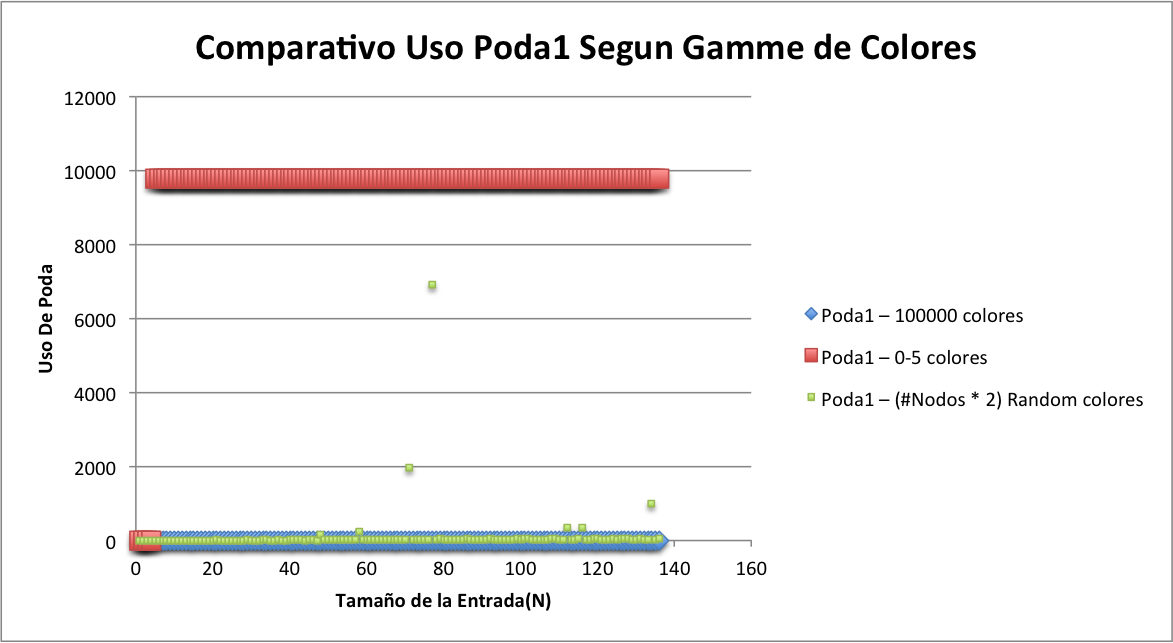
\includegraphics[width=140mm]{ejercicio2/ej2-comparativo-poda1-gammacolores.png}
\centering
\caption{Comparacion Uso de poda1 segun cantidad de colores posibles por nodo}
\label{overflow3}
\end{figure}\\
\pagebreak
Como podemos apreciar en el grafico, es muy claro que la poda1 solo sucede cuando la dispersion de colores es muy baja. Que quiere decir esto? Si nosotros tenemos muchos colores para elegir (por ejemplo un millon), es poco probable que tengamos un vecino que tenga un solo color disponible y que ademas sea el mismo en el cual estoy seteando el backtrack. Si la dispersion es baja, es mucho mas probable que nos encontremos con un color invalido(que ese color sea unico para algun vecino).\\
La conclusion que sacamos en que la poda1 se utiliza mucho siempre y cuando no tengamos una dispersion de colores muy grande.\\


\begin{figure}[h!]
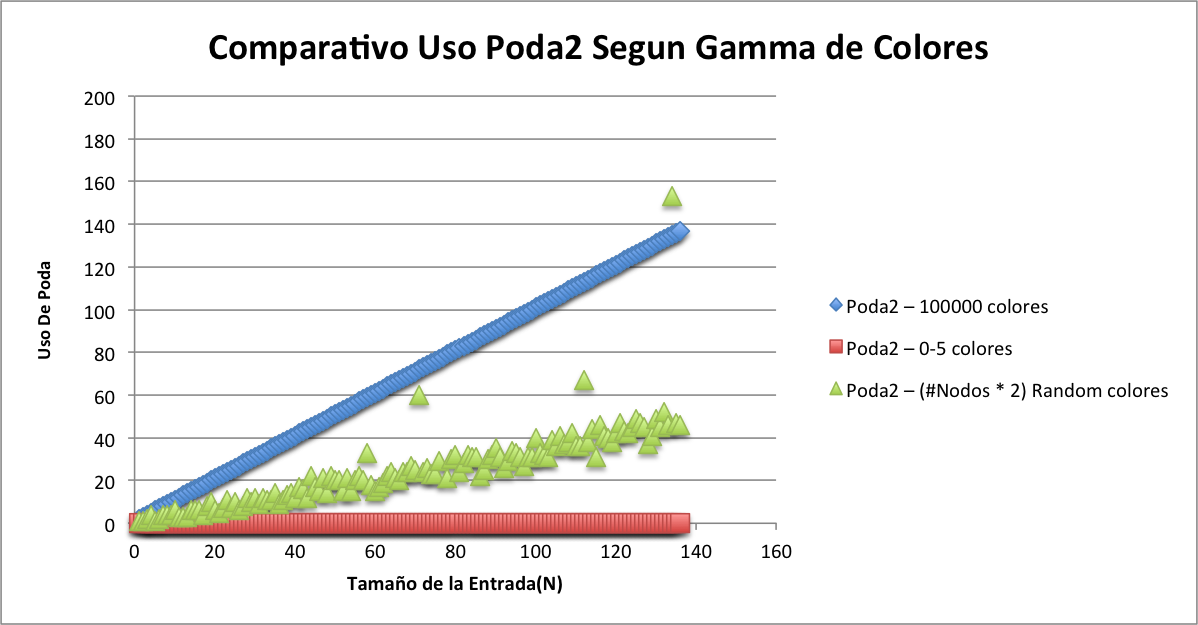
\includegraphics[width=140mm]{ejercicio2/ej2-comparativo-poda2-gammacolores.png}
\centering
\caption{Comparacion Uso de poda2 segun cantidad de colores posibles por nodo}
\label{overflow3}
\end{figure}\\

Este segundo grafico nos da la pauta de que sucede al reves que la anterior poda. Si los colores son muy dispersos, es probable que encontremos un color tal que ningun vecino mio lo contenga. Asimismo, si mi dispersion es muy baja, es altamente probable que los colores se repitan y no pueda descartar nada. En el medio tenemos la situacion donde tenemos una buena dispersion, sin embargo no es tan exagerada ni para un lado ni para el otro. De esa manera vemos que nuestro algoritmo utiliza mucho la poda2 siempre y cuando la variedad en la eleccion de los colores sea alta.\\|\\

\pagebreak
Ahora que sabemos que ambas podas son efectivas en cuanto a su uso, querriamos ver que sucede en cuanto al tiempo de ejecucion: si bien ambas se utilizan, es posible que ninguna o alguna de ellas no mejore visiblemente el tiempo de ejecucion.\\
En el siguiente grafo veremos los tiempos de ejecucion para un grafo cuyos colores no son dispersos

\begin{figure}[h!]
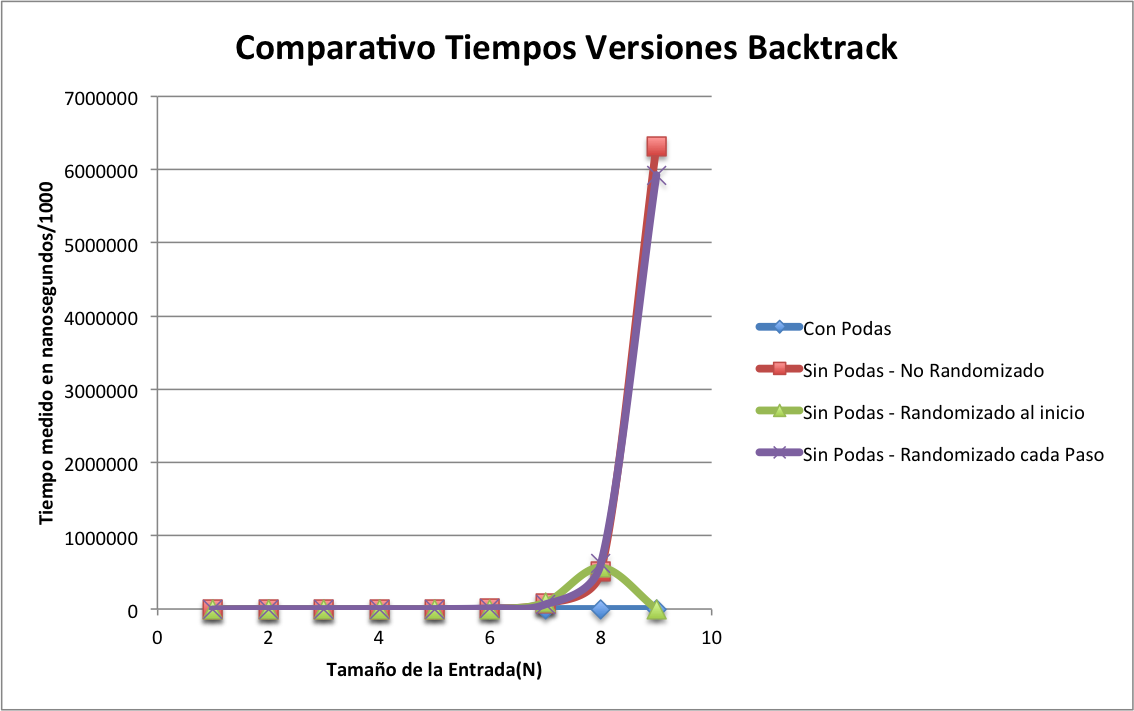
\includegraphics[width=140mm]{ejercicio2/ej2-comparativo-versionespng.png}
\centering
\caption{Comparacion Tiempos de ejecucion Poda vc No poda Colores no dispersos}
\label{overflow3}
\end{figure}
\\
\\

Lo que vemos es que si los colores estan poco distribuidos, el no utilizar la poda produce que los tiempos se vayan muy rapido hacia arriba. Siempre que utilicemos las podas el tiempo de ejecucion en comparacion a el tiempo versus sin podas es muchisimo menor. Asimismo vemos que justo el caso de color verde randomizo de una manera agradable y se acerco a la poda2 por ende su tiempo disminuyo considerablemente.\\

\pagebreak
Ahora veamos que sucede si tenemos los colores distribuidos:

\begin{figure}[h!]
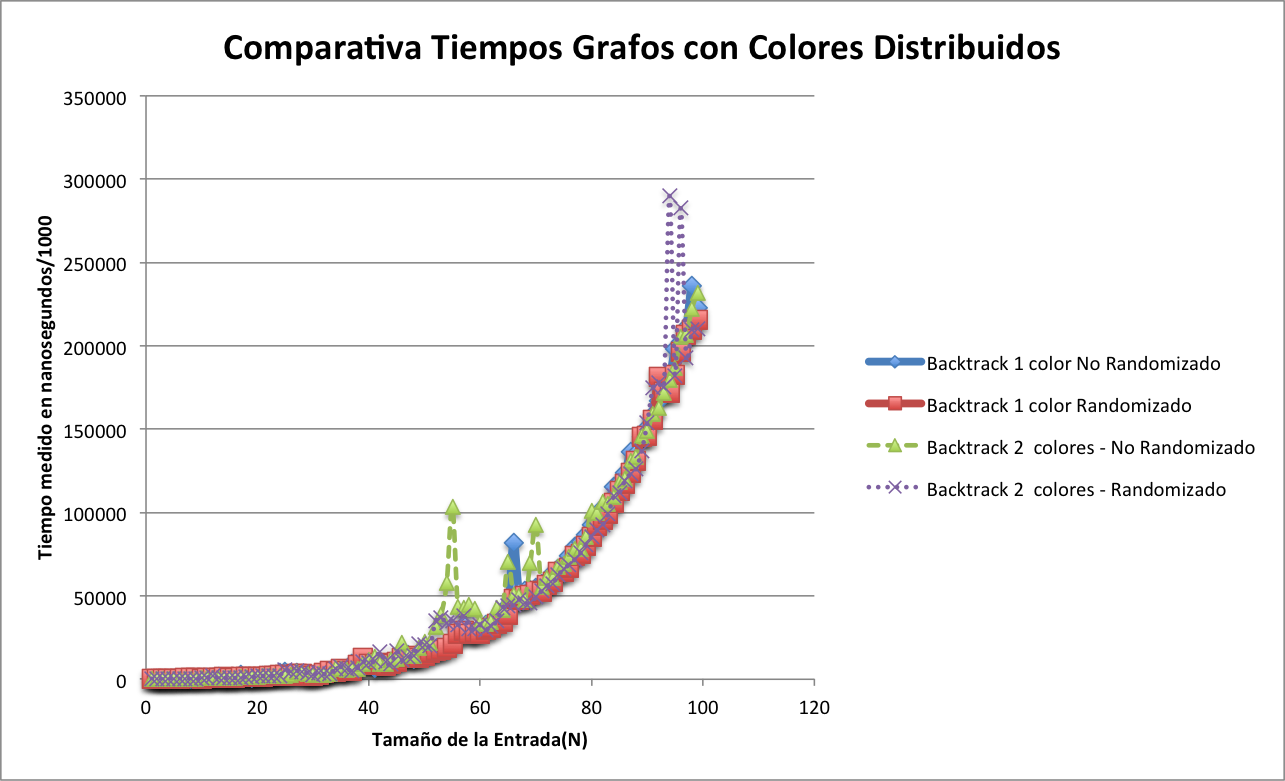
\includegraphics[width=140mm]{ejercicio2/ej2-comparativa-tiempos-colores-distribuidos.png}
\centering
\caption{Comparacion Uso de poda2 en relacion al tamanio de entrada(n+1 colores por nodo}
\label{overflow3}
\end{figure}

\\
\\
Lo que apreciamos es que si los colores estan distribuidos, entonces no importa que tipo de backtrack usemos. Si intentamos setear 2 colores para utilizar el ejercicio 1 o si o solo seeteamos 1 color para seguir con el backtrack, al tener los colores distribuidos, siempre entramos por la poda2, por lo que el tiempo de ejecucion se comparta mas o menos siempre de la misma manera. 
\pagebreak